\begin{figure}[h!]
	\centering
	
	
	
	\tikzset{every picture/.style={line width=0.75pt}} %set default line width to 0.75pt        
	
	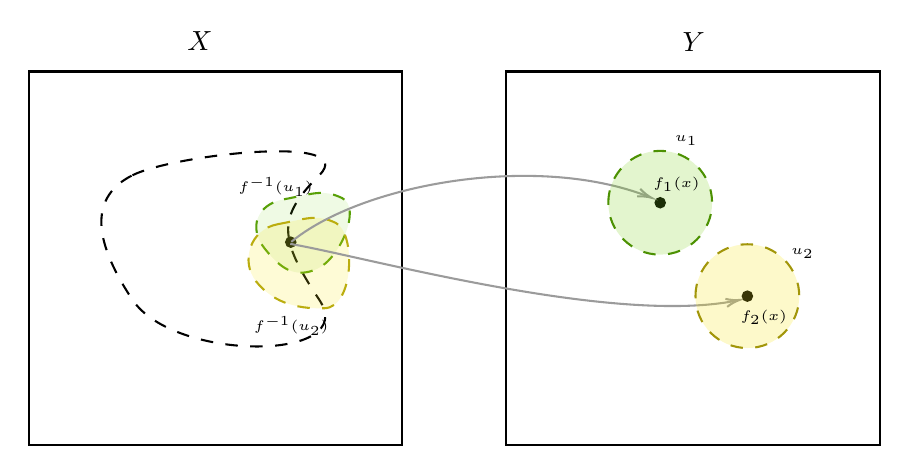
\begin{tikzpicture}[x=0.75pt,y=0.75pt,yscale=-1,xscale=1]
		%uncomment if require: \path (0,300); %set diagram left start at 0, and has height of 300
		
		%Shape: Circle [id:dp22945492936875378] 
		\draw  [fill={rgb, 255:red, 0; green, 0; blue, 0 }  ,fill opacity=1 ] (352,103.25) .. controls (352,102.01) and (353.01,101) .. (354.25,101) .. controls (355.49,101) and (356.5,102.01) .. (356.5,103.25) .. controls (356.5,104.49) and (355.49,105.5) .. (354.25,105.5) .. controls (353.01,105.5) and (352,104.49) .. (352,103.25) -- cycle ;
		%Shape: Square [id:dp934029333497959] 
		\draw   (50,40) -- (230,40) -- (230,220) -- (50,220) -- cycle ;
		%Shape: Square [id:dp16895777662650313] 
		\draw   (280,40) -- (460,40) -- (460,220) -- (280,220) -- cycle ;
		%Shape: Polygon Curved [id:ds9787457593928202] 
		\draw  [dash pattern={on 4.5pt off 4.5pt}] (100,90) .. controls (120,80) and (210,70) .. (190,90) .. controls (170,110) and (170,120) .. (190,150) .. controls (210,180) and (120,180) .. (100,150) .. controls (80,120) and (80,100) .. (100,90) -- cycle ;
		%Shape: Circle [id:dp057154404925263025] 
		\draw  [fill={rgb, 255:red, 0; green, 0; blue, 0 }  ,fill opacity=1 ] (174,122.25) .. controls (174,121.01) and (175.01,120) .. (176.25,120) .. controls (177.49,120) and (178.5,121.01) .. (178.5,122.25) .. controls (178.5,123.49) and (177.49,124.5) .. (176.25,124.5) .. controls (175.01,124.5) and (174,123.49) .. (174,122.25) -- cycle ;
		%Shape: Polygon Curved [id:ds5815057190055555] 
		\draw  [color={rgb, 255:red, 88; green, 160; blue, 7 }  ,draw opacity=1 ][fill={rgb, 255:red, 126; green, 211; blue, 33 }  ,fill opacity=0.12 ][dash pattern={on 4.5pt off 4.5pt}] (173,101.58) .. controls (186.5,99.08) and (191.5,96.42) .. (201,101) .. controls (210.5,105.58) and (200,130.08) .. (189,135.08) .. controls (178,140.08) and (171,134.58) .. (163.5,125.08) .. controls (156,115.58) and (159.5,104.08) .. (173,101.58) -- cycle ;
		%Shape: Polygon Curved [id:ds30989547801826567] 
		\draw  [color={rgb, 255:red, 187; green, 173; blue, 15 }  ,draw opacity=1 ][fill={rgb, 255:red, 248; green, 231; blue, 28 }  ,fill opacity=0.18 ][dash pattern={on 4.5pt off 4.5pt}] (170,113.58) .. controls (183.5,111.08) and (188.5,108.42) .. (198,113) .. controls (207.5,117.58) and (207,153.58) .. (192.5,154.08) .. controls (178,154.58) and (167,150.58) .. (159.5,141.08) .. controls (152,131.58) and (156.5,116.08) .. (170,113.58) -- cycle ;
		%Curve Lines [id:da29321026202366296] 
		\draw [color={rgb, 255:red, 155; green, 155; blue, 155 }  ,draw opacity=1 ][line width=0.75]    (176.5,122.08) .. controls (210.41,94.22) and (293.92,79.11) .. (348.36,100.19) ;
		\draw [shift={(350,100.84)}, rotate = 202.06] [color={rgb, 255:red, 155; green, 155; blue, 155 }  ,draw opacity=1 ][line width=0.75]    (6.56,-1.97) .. controls (4.17,-0.84) and (1.99,-0.18) .. (0,0) .. controls (1.99,0.18) and (4.17,0.84) .. (6.56,1.97)   ;
		%Curve Lines [id:da39067447551600165] 
		\draw [color={rgb, 255:red, 155; green, 155; blue, 155 }  ,draw opacity=1 ][line width=0.75]    (176,123.08) .. controls (211.15,129.02) and (330.58,162.4) .. (390.7,150.45) ;
		\draw [shift={(392.5,150.08)}, rotate = 167.68] [color={rgb, 255:red, 155; green, 155; blue, 155 }  ,draw opacity=1 ][line width=0.75]    (6.56,-1.97) .. controls (4.17,-0.84) and (1.99,-0.18) .. (0,0) .. controls (1.99,0.18) and (4.17,0.84) .. (6.56,1.97)   ;
		%Shape: Circle [id:dp16543584587564597] 
		\draw  [fill={rgb, 255:red, 0; green, 0; blue, 0 }  ,fill opacity=1 ] (394,148.25) .. controls (394,147.01) and (395.01,146) .. (396.25,146) .. controls (397.49,146) and (398.5,147.01) .. (398.5,148.25) .. controls (398.5,149.49) and (397.49,150.5) .. (396.25,150.5) .. controls (395.01,150.5) and (394,149.49) .. (394,148.25) -- cycle ;
		%Shape: Circle [id:dp376925694074147] 
		\draw  [color={rgb, 255:red, 76; green, 145; blue, 2 }  ,draw opacity=1 ][fill={rgb, 255:red, 126; green, 211; blue, 33 }  ,fill opacity=0.22 ][dash pattern={on 4.5pt off 4.5pt}] (329.25,103.25) .. controls (329.25,89.44) and (340.44,78.25) .. (354.25,78.25) .. controls (368.06,78.25) and (379.25,89.44) .. (379.25,103.25) .. controls (379.25,117.06) and (368.06,128.25) .. (354.25,128.25) .. controls (340.44,128.25) and (329.25,117.06) .. (329.25,103.25) -- cycle ;
		%Shape: Circle [id:dp3499499601701357] 
		\draw  [color={rgb, 255:red, 162; green, 150; blue, 10 }  ,draw opacity=1 ][fill={rgb, 255:red, 248; green, 231; blue, 28 }  ,fill opacity=0.23 ][dash pattern={on 4.5pt off 4.5pt}] (371.25,148.25) .. controls (371.25,134.44) and (382.44,123.25) .. (396.25,123.25) .. controls (410.06,123.25) and (421.25,134.44) .. (421.25,148.25) .. controls (421.25,162.06) and (410.06,173.25) .. (396.25,173.25) .. controls (382.44,173.25) and (371.25,162.06) .. (371.25,148.25) -- cycle ;
		
		% Text Node
		\draw (125,19.4) node [anchor=north west][inner sep=0.75pt]    {$X$};
		% Text Node
		\draw (363.5,19.9) node [anchor=north west][inner sep=0.75pt]    {$Y$};
		% Text Node
		\draw (349.5,89.4) node [anchor=north west][inner sep=0.75pt]  [font=\tiny]  {$f_{1}( x)$};
		% Text Node
		\draw (391.5,153.4) node [anchor=north west][inner sep=0.75pt]  [font=\tiny]  {$f_{2}( x)$};
		% Text Node
		\draw (360,69.4) node [anchor=north west][inner sep=0.75pt]  [font=\tiny]  {$u_{1}$};
		% Text Node
		\draw (416,123.9) node [anchor=north west][inner sep=0.75pt]  [font=\tiny]  {$u_{2}$};
		% Text Node
		\draw (149.5,89.4) node [anchor=north west][inner sep=0.75pt]  [font=\tiny]  {$f^{-1}( u_{1})$};
		% Text Node
		\draw (157,156.4) node [anchor=north west][inner sep=0.75pt]  [font=\tiny]  {$f^{-1}( u_{2})$};
		
		
	\end{tikzpicture}
\end{figure}